% ============================================================
%  يُترجَم بـ XeLaTeX  (في Overleaf: Menu → Compiler → XeLaTeX)
%  الخط: Amiri (متوفر في Overleaf، أو حمّله من github.com/aliftype/amiri)
% ============================================================
\documentclass[12pt,a4paper]{article}
\usepackage[a4paper,margin=1.7cm,top=2.3cm,bottom=2.9cm,headheight=15pt,footskip=1.5cm]{geometry}
\usepackage{amsmath,amssymb}
\usepackage{icomma}
\usepackage[english,bidi=default,layout=lists]{babel}
\babelprovide[import,main]{arabic}
\babelfont{rm}[Scale=1.08]{Amiri}
\babelfont{sf}[Scale=1.08]{Amiri}
\usepackage[most]{tcolorbox}
\usepackage{tikz}
\usetikzlibrary{arrows.meta,calc,shadings}
\usepackage{array}
\usepackage{colortbl}
\usepackage{fancyhdr}
\usepackage{titlesec}
\usepackage{enumitem}
\usepackage{collcell}
\usepackage{needspace}
\usepackage{etoolbox}
\newcolumntype{C}{>{\collectcell\ar}c<{\endcollectcell}}
\pretocmd{\section}{\Needspace{15\baselineskip}}{}{}
\pretocmd{\subsection}{\Needspace{11\baselineskip}}{}{}

\definecolor{cDef}{HTML}{1F4E9C}
\definecolor{cThm}{HTML}{B3261E}
\definecolor{cRem}{HTML}{2E7D32}
\definecolor{cEx}{HTML}{C76B00}
\definecolor{cMeth}{HTML}{6A1B9A}
\definecolor{cSol}{HTML}{00695C}
\definecolor{cSec}{HTML}{1F3A68}

\titleformat{\section}{\Large\bfseries\color{cSec}}{\thesection.}{0.6em}{}[{\color{cSec!60}\titlerule[1pt]}]
\titleformat{\subsection}{\large\bfseries\color{cThm!85!black}}{\thesubsection.}{0.5em}{}
\titlespacing*{\section}{0pt}{14pt}{8pt}
\titlespacing*{\subsection}{0pt}{10pt}{5pt}
\setlength{\parindent}{0pt}
\setlength{\parskip}{4pt}
\setlist{itemsep=2pt,topsep=3pt}

\newtcolorbox{arbox}[3][]{enhanced,
  colback=#2!5,colframe=#2!80!black,arc=2mm,boxrule=0.8pt,
  left=6pt,right=6pt,top=8pt,bottom=5pt,
  fonttitle=\bfseries,coltitle=white,
  title={\foreignlanguage{arabic}{#3}},
  attach boxed title to top right={xshift=-5mm,yshift=-3mm},
  boxed title style={colback=#2!80!black,arc=1.5mm,boxrule=0pt},
  before upper={\selectlanguage{arabic}},
  before skip=8pt,after skip=8pt,breakable,#1}
\newenvironment{BOX}[2]{\begin{otherlanguage}{english}\begin{arbox}{#1}{#2}}{\end{arbox}\end{otherlanguage}}
\newenvironment{tarif}[1][تعريف]{\begin{BOX}{cDef}{#1}}{\end{BOX}}
\newenvironment{khassia}[1][خاصية]{\begin{BOX}{cThm}{#1}}{\end{BOX}}
\newenvironment{molahada}[1][ملاحظة]{\begin{BOX}{cRem}{#1}}{\end{BOX}}
\newenvironment{mithal}[1][مثال]{\begin{BOX}{cEx}{#1}}{\end{BOX}}
\newenvironment{tariqa}[1][طريقة]{\begin{BOX}{cMeth}{#1}}{\end{BOX}}

\newcounter{exo}
\newenvironment{tamrin}[1]{\stepcounter{exo}\begin{BOX}{cSec}{التمرين \theexo: #1}}{\end{BOX}}
\newenvironment{hal}{\Needspace{12\baselineskip}\begin{otherlanguage}{english}\begin{arbox}[breakable]{cSol}{حل التمرين \theexo}}{\end{arbox}\end{otherlanguage}}

\newenvironment{LTR}{\begin{otherlanguage}{english}}{\end{otherlanguage}}
\newcommand{\ar}[1]{\foreignlanguage{arabic}{#1}}

\renewcommand{\dots}{\mathinner{\ldotp\ldotp\ldotp}}
\renewcommand{\ldots}{\mathinner{\ldotp\ldotp\ldotp}}
\renewcommand{\cdots}{\mathinner{\cdotp\cdotp\cdotp}}
\newcommand{\N}{\mathbb{N}}
\newcommand{\Z}{\mathbb{Z}}
\newcommand{\D}{\mathbb{D}}
\newcommand{\Q}{\mathbb{Q}}
\newcommand{\R}{\mathbb{R}}
\newcommand{\pgcd}{\operatorname{PGCD}}
\newcommand{\ppcm}{\operatorname{PPCM}}

% \NLseg{a}{b}{[}{]} ; \NLright{a}{[} ; \NLleft{b}{]}  (interval on a number line)
\newcommand{\NLseg}[4]{\begin{LTR}\begin{tikzpicture}[baseline=-0.6ex]
 \draw[-{Stealth[length=2mm]},gray!70](0,0)--(3.4,0);
 \draw[line width=2pt,cThm!80!black](0.7,0)--(2.7,0);
 \node[cThm!80!black,font=\LARGE] at (0.7,0){$#3$};
 \node[cThm!80!black,font=\LARGE] at (2.7,0){$#4$};
 \node[below=3pt,font=\footnotesize] at (0.7,0){$#1$};
 \node[below=3pt,font=\footnotesize] at (2.7,0){$#2$};
\end{tikzpicture}\end{LTR}}
\newcommand{\NLright}[2]{\begin{LTR}\begin{tikzpicture}[baseline=-0.6ex]
 \draw[-{Stealth[length=2mm]},gray!70](0,0)--(3.4,0);
 \draw[line width=2pt,cThm!80!black](1.3,0)--(3.3,0);
 \node[cThm!80!black,font=\LARGE] at (1.3,0){$#2$};
 \node[below=3pt,font=\footnotesize] at (1.3,0){$#1$};
\end{tikzpicture}\end{LTR}}
\newcommand{\NLleft}[2]{\begin{LTR}\begin{tikzpicture}[baseline=-0.6ex]
 \draw[-{Stealth[length=2mm]},gray!70](0,0)--(3.4,0);
 \draw[line width=2pt,cThm!80!black](0.05,0)--(2.1,0);
 \node[cThm!80!black,font=\LARGE] at (2.1,0){$#2$};
 \node[below=3pt,font=\footnotesize] at (2.1,0){$#1$};
\end{tikzpicture}\end{LTR}}

% ---------- social-media icons (pure TikZ) ----------
\definecolor{cFB}{HTML}{1877F2}
\definecolor{cTG}{HTML}{229ED9}
\definecolor{cIG1}{HTML}{FEDA75}
\definecolor{cIG2}{HTML}{D62976}
\definecolor{cIG3}{HTML}{4F5BD5}
\newcommand{\fbicon}{\begin{LTR}\begin{tikzpicture}[baseline=-0.75ex,x=1em,y=1em]
 \fill[cFB] (0,0) circle (0.55);
 \node[white,inner sep=0,font=\usefont{TU}{lmss}{bx}{n}\small] at (0.04,-0.02) {f};
\end{tikzpicture}\end{LTR}}
\newcommand{\igicon}{\begin{LTR}
\begin{tikzpicture}[baseline=-0.75ex,x=1em,y=1em]
 \shade[lower left=cIG1,lower right=cIG2,upper left=cIG2,upper right=cIG3,rounded corners=0.28em] (-0.55,-0.55) rectangle (0.55,0.55);
 \draw[white,line width=0.09em,rounded corners=0.18em] (-0.36,-0.36) rectangle (0.36,0.36);
 \draw[white,line width=0.09em] (0,0) circle (0.17);
 \fill[white] (0.22,0.22) circle (0.05);
\end{tikzpicture}\end{LTR}}
\newcommand{\tgicon}{\begin{LTR}
\begin{tikzpicture}[baseline=-0.75ex,x=1em,y=1em]
 \fill[cTG] (0,0) circle (0.55);
 \fill[white] (-0.33,0.0) -- (0.32,0.27) -- (0.2,-0.3) -- (0.0,-0.15) -- (-0.08,-0.28) -- (-0.08,-0.08) -- cycle;
 \fill[cTG!70!black] (-0.08,-0.08) -- (0.25,0.2) -- (0.0,-0.15) -- (-0.08,-0.28) -- cycle;
\end{tikzpicture}\end{LTR}}
% page number: black box, white two-digit number, at the right of the social row
\newcommand{\PageBox}{\begin{LTR}\tikz[baseline=(p.base)]\node[fill=black,text=white,inner sep=2.5pt,minimum width=1.6em,minimum height=1.3em,font=\usefont{TU}{lmss}{bx}{n}\small](p){\ifnum\value{page}<10 0\fi\arabic{page}};\end{LTR}}
% visual left-to-right order: Telegram | Instagram | Facebook | page box
\newcommand{\SocialRow}{\begin{otherlanguage}{english}%
 \ar{\textbf{الأستاذ سوايسية هشام للرياضيات}}\ \tgicon\hfill
 \textbf{prof\_hicham\_math}\ \igicon\hfill
 \ar{\textbf{الأستاذ سوايسية هشام للرياضيات}}\ \fbicon\hspace{2.2em}\PageBox\end{otherlanguage}}

\pagestyle{fancy}
\fancyhf{}
\renewcommand{\headrulewidth}{0.6pt}
\renewcommand{\footrulewidth}{0.4pt}
% \SetHeader{right head: document title}{left head: level -- stream}
\newcommand{\SetHeader}[2]{%
 \fancyhead[C]{\parbox{\textwidth}{\ar{#1\hfill #2}}}%
 \fancyfoot[C]{\parbox{\textwidth}{\small\SocialRow}}}
\usepackage{tkz-tab}
\usepackage{multicol}
% variation / sign table (LTR)
\newenvironment{TAB}{\par\begin{center}\begin{LTR}\begin{tikzpicture}[scale=0.95,every node/.style={font=\small}]}{\end{tikzpicture}\end{LTR}\end{center}}
% grid + axes, clipped: \begin{GR}{xmin}{xmax}{ymin}{ymax}{unit cm}
\newenvironment{GR}[5]{\par\begin{center}\begin{LTR}\begin{tikzpicture}[x=#5cm,y=#5cm,font=\footnotesize]
 \draw[gray!25,very thin] (#1,#3) grid (#2,#4);
 \draw[-{Stealth[length=2mm]}] (#1,0)--(#2+0.3,0) node[below left]{$x$};
 \draw[-{Stealth[length=2mm]}] (0,#3)--(0,#4+0.3) node[below left]{$y$};
 \node[below left] at (0,0){$O$};
 \begin{scope}\clip (#1,#3) rectangle (#2,#4);}
{\end{scope}\end{tikzpicture}\end{LTR}\end{center}}
\newcommand{\Ticks}[2]{\foreach \t in {#1} \node[below,font=\scriptsize] at (\t,0){$\t$}; \foreach \t in {#2} \node[left,font=\scriptsize] at (0,\t){$\t$};}
\newcommand{\bx}[1]{\ensuremath{\colorbox{cDef!12}{$\displaystyle #1$}}}
\newcommand{\TwoCol}[4]{\par\begin{LTR}\noindent\begin{minipage}[t]{#1\textwidth}\selectlanguage{arabic}#2\end{minipage}\hfill\begin{minipage}[t]{#3\textwidth}\selectlanguage{arabic}#4\end{minipage}\end{LTR}\par}
\newcommand{\RL}[4]{\TwoCol{#3}{#4}{#1}{#2}}  % \RL{w1}{right content}{w2}{left content}
\newcommand{\ok}{$\textcolor{cRem}{\checkmark}$}
\newcommand{\limn}{\displaystyle\lim_{n\to+\infty}}
% sub-questions, each on its own line
\newenvironment{sq}{\begin{itemize}[leftmargin=2.4em,itemsep=3pt]}{\end{itemize}}
\newcommand{\qa}{\item[(أ)]}\newcommand{\qb}{\item[(ب)]}\newcommand{\qc}{\item[(جـ)]}\newcommand{\qd}{\item[(د)]}\newcommand{\qe}{\item[(هـ)]}
\newcommand{\pa}{\par\smallskip\textbf{(أ)} }\newcommand{\pb}{\par\smallskip\textbf{(ب)} }\newcommand{\pc}{\par\smallskip\textbf{(جـ)} }\newcommand{\pd}{\par\smallskip\textbf{(د)} }\newcommand{\pe}{\par\smallskip\textbf{(هـ)} }
\newcommand{\QQ}[1]{\par\smallskip\textbf{#1.} }
\newenvironment{tmr}{\stepcounter{exo}\begin{BOX}{cSec}{تمرين محلول \theexo}}{\end{BOX}}
\newcommand{\ABC}[3]{\\[2pt]\begin{tabular}{p{0.28\textwidth}p{0.28\textwidth}p{0.28\textwidth}}(جـ) \ #3 & (ب) \ #2 & (أ) \ #1\end{tabular}}
\pretocmd{\section}{\Needspace{24\baselineskip}}{}{}
\newtcbox{\bxtbox}{on line,colback=cDef!12,colframe=cDef!12,boxrule=0pt,arc=1pt,boxsep=0pt,left=2pt,right=2pt,top=1pt,bottom=1pt}
\newcommand{\bxt}[1]{\foreignlanguage{english}{\bxtbox{\ar{#1}}}}
\renewcommand{\bx}[1]{\ensuremath{\colorbox{cDef!12}{$\displaystyle\color{cThm}#1$}}}
\renewcommand{\bxt}[1]{\foreignlanguage{english}{\bxtbox{\ar{\color{cThm}#1}}}}
\newcommand{\LW}[1]{{\color{cDef}#1}}
\newcommand{\ck}{\ensuremath{{\color{cRem}\checkmark}}}
% ---------- أشكال الفضاء (منظور متساوي القياس) ----------
% \CubeFig{scale}{extra tikz}: مكعب ABCDEFGH ، الأحرف المخفية متقطعة
\newcommand{\CubeFig}[2]{\begin{LTR}\begin{tikzpicture}[scale=#1,font=\small,line join=round]
\coordinate (A) at (0,0); \coordinate (B) at (2,0); \coordinate (C) at (2.9,0.8); \coordinate (D) at (0.9,0.8);
\coordinate (E) at (0,2); \coordinate (F) at (2,2); \coordinate (G) at (2.9,2.8); \coordinate (H) at (0.9,2.8);
\draw[thick] (A)--(B)--(F)--(E)--cycle; \draw[thick] (B)--(C)--(G)--(F); \draw[thick] (E)--(H)--(G);
\draw[dashed] (A)--(D)--(C); \draw[dashed] (D)--(H);
#2
\foreach \p/\pos in {A/below left,B/below right,C/right,D/left,E/left,F/below right,G/above right,H/above left} \node[\pos] at (\p){$\p$};
\end{tikzpicture}\end{LTR}}
% متوازي مستطيلات بأبعاد a (عرض) b (عمق) c (ارتفاع)
\newcommand{\BoxFig}[4]{\begin{LTR}\begin{tikzpicture}[scale=#4,font=\small,line join=round]
\coordinate (A) at (0,0); \coordinate (B) at (#1,0); \coordinate (C) at ({#1+0.45*#2},{0.4*#2}); \coordinate (D) at ({0.45*#2},{0.4*#2});
\coordinate (E) at (0,#3); \coordinate (F) at (#1,#3); \coordinate (G) at ({#1+0.45*#2},{#3+0.4*#2}); \coordinate (H) at ({0.45*#2},{#3+0.4*#2});
\draw[thick] (A)--(B)--(F)--(E)--cycle; \draw[thick] (B)--(C)--(G)--(F); \draw[thick] (E)--(H)--(G);
\draw[dashed] (A)--(D)--(C); \draw[dashed] (D)--(H);
\node[below] at ($(A)!0.5!(B)$){$a$}; \node[below right] at ($(B)!0.5!(C)$){$b$}; \node[left] at ($(A)!0.5!(E)$){$c$};
\end{tikzpicture}\end{LTR}}
\newcommand{\CylFig}{\begin{LTR}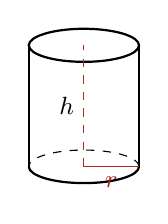
\begin{tikzpicture}[scale=0.7,font=\small]
\draw[thick] (-1,0) arc (180:360:1 and 0.3); \draw[dashed] (1,0) arc (0:180:1 and 0.3);
\draw[thick] (0,2.2) ellipse (1 and 0.3); \draw[thick] (-1,0)--(-1,2.2); \draw[thick] (1,0)--(1,2.2);
\draw[cThm] (0,0)--(1,0) node[midway,below]{$r$}; \draw[cThm,dashed] (0,0)--(0,2.2); \node[left] at (0,1.1){$h$};
\end{tikzpicture}\end{LTR}}
\newcommand{\ConeFig}{\begin{LTR}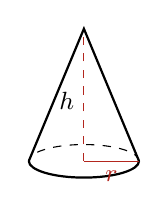
\begin{tikzpicture}[scale=0.7,font=\small]
\draw[thick] (-1,0) arc (180:360:1 and 0.3); \draw[dashed] (1,0) arc (0:180:1 and 0.3);
\draw[thick] (-1,0)--(0,2.4)--(1,0);
\draw[cThm] (0,0)--(1,0) node[midway,below]{$r$}; \draw[cThm,dashed] (0,0)--(0,2.4); \node[left] at (0,1.1){$h$};
\end{tikzpicture}\end{LTR}}
\newcommand{\SphFig}{\begin{LTR}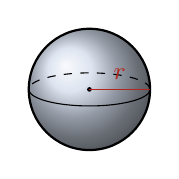
\begin{tikzpicture}[scale=0.7,font=\small]
\shade[ball color=cDef!20] (0,0) circle (1.1); \draw[thick] (0,0) circle (1.1);
\draw (-1.1,0) arc (180:360:1.1 and 0.3); \draw[dashed] (1.1,0) arc (0:180:1.1 and 0.3);
\fill (0,0) circle (1.2pt); \draw[cThm] (0,0)--(1.1,0) node[midway,above]{$r$};
\end{tikzpicture}\end{LTR}}
% هرم رباعي SABCD قاعدته مربع ومركزها O
\newcommand{\PyrFig}[1]{\begin{LTR}\begin{tikzpicture}[scale=#1,font=\small,line join=round]
\coordinate (A) at (0,0); \coordinate (B) at (2.4,0); \coordinate (C) at (3.3,0.9); \coordinate (D) at (0.9,0.9);
\coordinate (O) at (1.65,0.45); \coordinate (S) at (1.65,2.8); \coordinate (I) at ($(B)!0.5!(C)$);
\draw[thick] (A)--(B)--(C); \draw[dashed] (C)--(D)--(A); \draw[thick] (S)--(A); \draw[thick] (S)--(B); \draw[thick] (S)--(C); \draw[dashed] (S)--(D);
\draw[dashed,cThm] (S)--(O); \draw[dashed] (A)--(C); \draw[dashed] (B)--(D); \draw[cRem] (S)--(I);
\foreach \p/\pos in {A/below left,B/below right,C/right,D/left,S/above,O/below,I/right} \node[\pos] at (\p){$\p$};
\end{tikzpicture}\end{LTR}}
\relpenalty=10000\binoppenalty=10000\tolerance=9000\emergencystretch=0.3\linewidth
\SetHeader{\small\bfseries\color{cSec}تمارين: الهندسة في الفضاء}{\small\color{cSec}السنة الأولى ثانوي -- جذع مشترك علوم وتكنولوجيا}
\begin{document}
\begin{LTR}
\begin{tcolorbox}[enhanced,colback=cSec!10,colframe=cSec!40,arc=3mm,halign=center,boxrule=0.6pt,top=12pt,bottom=12pt,before upper={\selectlanguage{arabic}}]
{\color{cSec}\fontsize{26}{32}\selectfont\bfseries سلسلة تمارين: الهندسة في الفضاء}\\[8pt]
{\color{cSec!80!black}\large تمارين متدرجة ومسائل مع الحلول المفصلة}\\[5pt]
{\color{cSec!80!black}\large السنة الأولى ثانوي -- جذع مشترك علوم وتكنولوجيا}
\end{tcolorbox}
\end{LTR}

% =====================================================================
\section{المجسمات المألوفة: الأطوال والمساحات والحجوم}
\begin{tamrin}{تطبيق مباشر للدساتير}
احسب المساحة والحجم في كل حالة:
\begin{enumerate}
\item مكعب طول حرفه $5\,\mathrm{cm}$.
\item متوازي مستطيلات أبعاده $6\,\mathrm{cm}$ ، $4\,\mathrm{cm}$ و $3\,\mathrm{cm}$.
\item أسطوانة قائمة نصف قطرها $3\,\mathrm{cm}$ وارتفاعها $8\,\mathrm{cm}$ (المساحة الجانبية والكلية).
\item كرة نصف قطرها $6\,\mathrm{cm}$.
\item مخروط دوراني نصف قطر قاعدته $3\,\mathrm{cm}$ وارتفاعه $4\,\mathrm{cm}$ (الحجم فقط).
\end{enumerate}
\end{tamrin}
\begin{hal}
\QQ{1} $\mathcal A=6\times5^2=\bx{150\ \mathrm{cm}^2}$ \quad ؛ \quad $V=5^3=\bx{125\ \mathrm{cm}^3}$.
\QQ{2} $\mathcal A=2(6\times4+4\times3+3\times6)=2(24+12+18)=\bx{108\ \mathrm{cm}^2}$ \quad ؛ \quad $V=6\times4\times3=\bx{72\ \mathrm{cm}^3}$.
\QQ{3} الجانبية: $2\pi\times3\times8=\bx{48\pi\ \mathrm{cm}^2}$.\par
الكلية: $48\pi+2\times\pi\times3^2=48\pi+18\pi=\bx{66\pi\approx207{,}3\ \mathrm{cm}^2}$.\par
الحجم: $\pi\times3^2\times8=\bx{72\pi\approx226{,}2\ \mathrm{cm}^3}$.
\QQ{4} $\mathcal A=4\pi\times6^2=\bx{144\pi\ \mathrm{cm}^2}$ \quad ؛ \quad $V=\dfrac43\pi\times6^3=\bx{288\pi\ \mathrm{cm}^3}$.
\QQ{5} $V=\dfrac13\pi\times3^2\times4=\bx{12\pi\approx37{,}7\ \mathrm{cm}^3}$.
\end{hal}

\begin{tamrin}{حوض سمك (وضعية من الواقع)}
حوض سمك على شكل متوازي مستطيلات أبعاده الداخلية: الطول $50\,\mathrm{cm}$ ، العرض $30\,\mathrm{cm}$ والارتفاع $40\,\mathrm{cm}$.
\begin{enumerate}
\item احسب سعة الحوض باللتر.
\item نملأ الحوض بالماء إلى $\dfrac34$ ارتفاعه. ما كمية الماء باللتر؟
\item نضع فيه حجرًا فيرتفع مستوى الماء بـ $2\,\mathrm{cm}$. ما حجم الحجر؟
\end{enumerate}
\end{tamrin}
\begin{hal}
\QQ{1} $V=50\times30\times40=60000\ \mathrm{cm}^3$. وبما أن $1\,\mathrm{L}=1000\,\mathrm{cm}^3$: \quad السعة \bx{60\ \mathrm{L}}.
\QQ{2} ارتفاع الماء $\dfrac34\times40=30\,\mathrm{cm}$ ، إذن $V=50\times30\times30=45000\ \mathrm{cm}^3=\bx{45\ \mathrm{L}}$.
\QQ{3} حجم الحجر يساوي حجم الماء المُزاح: $50\times30\times2=\bx{3000\ \mathrm{cm}^3}$ أي $3\,\mathrm{L}$.
\end{hal}

\begin{tamrin}{خزان ماء أسطواني}
خزان ماء على شكل أسطوانة قائمة نصف قطر قاعدتها $1\,\mathrm{m}$ وارتفاعها $2\,\mathrm{m}$.
\begin{enumerate}
\item احسب حجم الخزان بـ $\mathrm{m}^3$ ثم باللتر (تدوير إلى الوحدة).
\item نريد طلاء سطحه الجانبي فقط. احسب المساحة المطلية (تدوير إلى $0{,}01$).
\item يستهلك العامل $0{,}25\,\mathrm{L}$ من الطلاء لكل $1\,\mathrm{m}^2$. كم لترًا يحتاج؟
\end{enumerate}
\end{tamrin}
\begin{hal}
\QQ{1} $V=\pi\times1^2\times2=2\pi\approx6{,}283\ \mathrm{m}^3$ ، و $1\,\mathrm{m}^3=1000\,\mathrm{L}$: \quad $V\approx\bx{6283\ \mathrm{L}}$.
\QQ{2} $\mathcal A=2\pi\times1\times2=4\pi\approx\bx{12{,}57\ \mathrm{m}^2}$.
\QQ{3} $12{,}57\times0{,}25\approx\bx{3{,}14\ \mathrm{L}}$.
\end{hal}

\begin{tamrin}{مجسم مركّب}
مجسم مكوَّن من مكعب $ABCDEFGH$ طول حرفه $6\,\mathrm{cm}$ ، يعلوه هرم $SEFGH$ قاعدته الوجه $EFGH$ ورأسه $S$ ، ارتفاعه $SO'=4\,\mathrm{cm}$ حيث $O'$ مركز المربع $EFGH$.
\begin{enumerate}
\item احسب حجم المجسم.
\item ليكن $I$ منتصف $[FG]$. احسب $O'I$ ثم $SI$.
\item احسب المساحة الكلية للمجسم.
\item احسب طول الحرف $SF$.
\end{enumerate}
\end{tamrin}
\begin{hal}
\QQ{1} $V=6^3+\dfrac13\times6^2\times4=216+48=\bx{264\ \mathrm{cm}^3}$.
\QQ{2} $O'$ مركز المربع ، إذن $O'I$ يساوي نصف طول الضلع: $O'I=\bx{3\ \mathrm{cm}}$.\par
$(SO')$ عمودي على المستوي $(EFG)$ ، إذن $(SO')\perp(O'I)$ ، والمثلث $SO'I$ قائم في $O'$:\par
$SI^2=4^2+3^2=25$ \quad ومنه \quad $SI=\bx{5\ \mathrm{cm}}$.
\QQ{3} الوجه $EFGH$ مخفي. المساحة = خمسة أوجه للمكعب + أربعة مثلثات متقايسة:\par
$\mathcal A=5\times36+4\times\dfrac{6\times5}2=180+60=\bx{240\ \mathrm{cm}^2}$.
\QQ{4} $(SI)\perp(FG)$ لأن المثلث $SFG$ متساوي الساقين و $I$ منتصف $[FG]$ ، فالمثلث $SIF$ قائم في $I$:\par
$SF^2=5^2+3^2=34$ \quad ومنه \quad $SF=\bx{\sqrt{34}\approx5{,}83\ \mathrm{cm}}$.
\end{hal}

\begin{tamrin}{كرة داخل مكعب}
كرة محاطة داخل مكعب طول حرفه $10\,\mathrm{cm}$ (تمس أوجهه الستة).
\begin{enumerate}
\item ما نصف قطر الكرة؟
\item احسب حجم الكرة (تدوير إلى $0{,}1$).
\item ما النسبة المئوية من حجم المكعب التي تشغلها الكرة؟
\end{enumerate}
\end{tamrin}
\begin{hal}
\QQ{1} قطر الكرة يساوي حرف المكعب: $2r=10$ ، إذن \bx{r=5\ \mathrm{cm}}.
\QQ{2} $V=\dfrac43\pi\times5^3=\dfrac{500\pi}3\approx\bx{523{,}6\ \mathrm{cm}^3}$.
\QQ{3} $\dfrac{500\pi/3}{1000}=\dfrac\pi6\approx0{,}524$ ، أي حوالي \bx{52{,}4\,\%}.
\end{hal}

% =====================================================================
\section{التصميم والمنظور متساوي القياس}
\begin{tamrin}{تصميم ومساحة}
\begin{enumerate}
\item ارسم تصميم متوازي مستطيلات أبعاده $3\,\mathrm{cm}$ ، $2\,\mathrm{cm}$ و $1\,\mathrm{cm}$ ، ثم احسب مساحة التصميم.
\item ارسم بالمنظور متساوي القياس مكعبًا $ABCDEFGH$ طول حرفه $3\,\mathrm{cm}$.
\item تصميم أسطوانة قائمة مستطيل بعداه $12{,}56\,\mathrm{cm}$ و $5\,\mathrm{cm}$ وقرصان. احسب نصف قطر القرص (خذ $\pi\approx3{,}14$).
\end{enumerate}
\end{tamrin}
\begin{hal}
\QQ{1} التصميم ستة مستطيلات: اثنان $3\times2$ ، اثنان $2\times1$ ، اثنان $3\times1$ ، مرتبة بحيث تنطبق عند الطي.
\begin{LTR}\begin{center}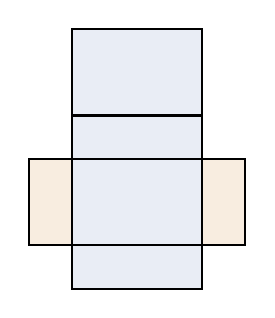
\begin{tikzpicture}[scale=0.55]
\draw[thick,fill=cDef!10] (0,0) rectangle (3,2); \draw[thick,fill=cDef!10] (0,2) rectangle (3,3);
\draw[thick,fill=cDef!10] (0,3) rectangle (3,5); \draw[thick,fill=cDef!10] (0,-1) rectangle (3,0);
\draw[thick,fill=cEx!12] (-1,0) rectangle (0,2); \draw[thick,fill=cEx!12] (3,0) rectangle (4,2);
\end{tikzpicture}\end{center}\end{LTR}
مساحة التصميم = مساحة المجسم: $2(3\times2+2\times1+3\times1)=2(6+2+3)=\bx{22\ \mathrm{cm}^2}$.
\QQ{2} نرسم الوجه الأمامي $ABFE$ مربعًا بأبعاده الحقيقية ، والأحرف $[AD]$ ، $[BC]$ ، $[FG]$ ، $[EH]$ مائلة ومتوازية وبطول مُصغَّر ، والأحرف المخفية متقطعة:
\begin{center}\CubeFig{0.8}{}\end{center}
\QQ{3} طول المستطيل هو محيط القاعدة: $2\pi r=12{,}56$ ، إذن $r=\dfrac{12{,}56}{2\times3{,}14}=\bx{2\ \mathrm{cm}}$.
\end{hal}

% =====================================================================
\section{الأوضاع النسبية}
\begin{tamrin}{مستقيمان في مكعب}
$ABCDEFGH$ مكعب. عيّن الوضع النسبي لكل مستقيمين (متقاطعان ، متوازيان ، ليسا من نفس المستوي) مع التبرير:
\begin{sq}
\qa $(AB)$ و $(HG)$.
\qb $(AB)$ و $(CG)$.
\qc $(AC)$ و $(BD)$.
\qd $(EG)$ و $(AC)$.
\qe $(BH)$ و $(DF)$.
\end{sq}
\end{tamrin}
\begin{hal}
\begin{center}\CubeFig{0.85}{\draw[cThm,thick] (B)--(H); \draw[cDef,thick] (D)--(F);}\end{center}
\pa $(AB)\parallel(DC)$ و $(DC)\parallel(HG)$ ، إذن \bxt{$(AB)$ و $(HG)$ متوازيان}.
\pb $(CG)$ يقطع المستوي $(ABC)$ في $C$ فقط ، و $C\notin(AB)$ ، فلا يمكن أن يتقاطعا ؛ ولا يتوازيان لأن $(CG)$ يقطع $(ABC)$. إذن \bxt{ليسا من نفس المستوي}.
\pc قطرا المربع $ABCD$: \bxt{متقاطعان في مركزه}.
\pd $AE=CG$ و $(AE)\parallel(CG)$ ، إذن $ACGE$ متوازي أضلاع: \bxt{$(EG)$ و $(AC)$ متوازيان}.
\pe $(BF)\parallel(DH)$ و $BF=DH$ ، إذن $BDHF$ متوازي أضلاع ، و $[BH]$ و $[DF]$ قطراه: \bxt{متقاطعان في منتصفهما}.
\end{hal}

\begin{tamrin}{مستقيم ومستوٍ ، مستويان}
$ABCDEFGH$ مكعب ، $O$ مركز الوجه $ABCD$ و $O'$ مركز الوجه $EFGH$.
\begin{enumerate}
\item عيّن الوضع النسبي للمستقيم والمستوي: \quad $(FH)$ و $(ABC)$ \quad ؛ \quad $(AG)$ و $(ABC)$ \quad ؛ \quad $(BD)$ و $(ABC)$.
\item عيّن تقاطع المستويين $(ABFE)$ و $(BCGF)$.
\item عيّن تقاطع المستويين $(ACGE)$ و $(BDHF)$.
\item ما الوضع النسبي للمستويين $(ABCD)$ و $(EFGH)$ ؟
\end{enumerate}
\end{tamrin}
\begin{hal}
\QQ{1} $(FH)\parallel(BD)$ (لأن $BDHF$ متوازي أضلاع) و $(BD)\subset(ABC)$ ، و $F\notin(ABC)$: \bxt{$(FH)$ يوازي $(ABC)$ تمامًا}.\par
$(AG)$ يشمل $A\in(ABC)$ و $G\notin(ABC)$: \bxt{$(AG)$ يقطع $(ABC)$ في النقطة $A$}.\par
$B$ و $D$ من $(ABC)$: \bxt{$(BD)$ محتوى في $(ABC)$}.
\QQ{2} $B$ و $F$ مشتركتان بين المستويين ، والمستويان غير منطبقين: \bxt{تقاطعهما المستقيم $(BF)$}.
\QQ{3} $O\in(AC)\subset(ACGE)$ و $O\in(BD)\subset(BDHF)$ ، فهي مشتركة ؛ وبنفس الطريقة $O'$ مشتركة: \bxt{تقاطعهما المستقيم $(OO')$}.
\QQ{4} الوجهان المتقابلان لمكعب في مستويين \bxt{متوازيين تمامًا}.
\end{hal}

\begin{tamrin}{صحيح أم خطأ}
أجب بـ «صحيح» أو «خطأ» مع التبرير:
\begin{enumerate}
\item مستقيمان لا يتقاطعان في الفضاء متوازيان.
\item من ثلاث نقط في الفضاء يمر دائمًا مستوٍ وحيد.
\item إذا وازى مستقيم مستويًا فإنه يوازي كل مستقيمات هذا المستوي.
\item مستقيمان موازيان لمستقيم ثالث متوازيان.
\item مستويان لهما نقطتان مشتركتان متمايزتان متقاطعان أو منطبقان.
\end{enumerate}
\end{tamrin}
\begin{hal}
\QQ{1} \bxt{خطأ}: في المكعب $(AE)$ و $(BC)$ لا يتقاطعان ولا يتوازيان.
\QQ{2} \bxt{خطأ}: يجب أن تكون النقط الثلاث ليست على استقامة واحدة ؛ وإلا مر بها عدد لا نهائي من المستويات.
\QQ{3} \bxt{خطأ}: $(EF)$ يوازي $(ABCD)$ لكنه لا يوازي $(BC)$.
\QQ{4} \bxt{صحيح}: مبرهنة التوازي في الفضاء.
\QQ{5} \bxt{صحيح}: يشمل كل منهما المستقيم الذي يمر بالنقطتين ، فإما ينطبقان وإما يتقاطعان وفق هذا المستقيم.
\end{hal}

% =====================================================================
\section{التوازي والتعامد في الفضاء}
\begin{tamrin}{مستويان متوازيان في مكعب}
$ABCDEFGH$ مكعب.
\begin{enumerate}
\item بيّن أن $ADGF$ متوازي أضلاع ، واستنتج أن $(AF)\parallel(DG)$.
\item بيّن بنفس الطريقة أن $(AH)\parallel(BG)$.
\item استنتج أن المستويين $(AFH)$ و $(BDG)$ متوازيان.
\end{enumerate}
\end{tamrin}
\begin{hal}
\begin{center}\CubeFig{0.85}{\draw[cThm,thick] (A)--(F)--(H)--cycle; \draw[cDef,thick,dashed] (B)--(D); \draw[cDef,thick] (D)--(G)--(B);}\end{center}
\QQ{1} $(AD)\parallel(BC)\parallel(FG)$ و $AD=FG$ ، إذن الرباعي $ADGF$ متوازي أضلاع ، ومنه \bxt{$(AF)\parallel(DG)$}.
\QQ{2} $(AB)\parallel(HG)$ و $AB=HG$ ، إذن $ABGH$ متوازي أضلاع ، ومنه \bxt{$(AH)\parallel(BG)$}.
\QQ{3} المستقيمان $(AF)$ و $(AH)$ متقاطعان في $A$ ومحتويان في $(AFH)$ ؛\par
$(AF)\parallel(DG)$ و $(DG)\subset(BDG)$ ، إذن $(AF)$ يوازي $(BDG)$ ؛ وكذلك $(AH)\parallel(BG)$ فـ $(AH)$ يوازي $(BDG)$.\par
مستقيمان متقاطعان من $(AFH)$ يوازيان $(BDG)$ ، إذن \bxt{المستويان $(AFH)$ و $(BDG)$ متوازيان}.
\end{hal}

\begin{tamrin}{تعامد وحساب أطوال في مكعب}
$ABCDEFGH$ مكعب طول حرفه $a$.
\begin{enumerate}
\item بيّن أن $(AE)$ عمودي على المستوي $(ABCD)$ ، واستنتج أن المثلث $AEC$ قائم.
\item احسب $AC$ ثم $EC$ بدلالة $a$.
\item احسب حجم رباعي الوجوه $ABDE$.
\item بيّن أن المثلث $BDE$ متقايس الأضلاع ، واحسب مساحته.
\item استنتج المسافة من $A$ إلى المستوي $(BDE)$.
\end{enumerate}
\end{tamrin}
\begin{hal}
\QQ{1} $(AE)\perp(AB)$ و $(AE)\perp(AD)$ (أوجه مربعة) ، و $(AB)$ و $(AD)$ متقاطعان في المستوي $(ABCD)$ ، إذن \bxt{$(AE)$ عمودي على $(ABCD)$}.\par
بما أن $(AC)\subset(ABCD)$ فإن $(AE)\perp(AC)$: \bxt{المثلث $AEC$ قائم في $A$}.
\QQ{2} في المربع $ABCD$: $AC=\bx{a\sqrt2}$. \quad وفي المثلث $AEC$: $EC^2=a^2+2a^2=3a^2$ ، إذن $EC=\bx{a\sqrt3}$.
\QQ{3} نعتبر القاعدة المثلث $ABD$ (مساحته $\dfrac{a^2}2$) والارتفاع $AE=a$:\par
$V=\dfrac13\times\dfrac{a^2}2\times a=\bx{\dfrac{a^3}6}$.
\QQ{4} $BD$ ، $DE$ و $EB$ أقطار لأوجه المكعب ، طول كل منها $a\sqrt2$: المثلث $BDE$ \bxt{متقايس الأضلاع}.\par
مساحة مثلث متقايس الأضلاع طول ضلعه $c$ هي $\dfrac{\sqrt3}4c^2$ ، إذن $\mathcal A=\dfrac{\sqrt3}4\times2a^2=\bx{\dfrac{\sqrt3}2a^2}$.
\QQ{5} نحسب الحجم نفسه بقاعدة $BDE$ وارتفاع $d$ (المسافة من $A$ إلى المستوي):\par
$\dfrac13\times\dfrac{\sqrt3}2a^2\times d=\dfrac{a^3}6$ \quad ومنه \quad $d=\dfrac{a}{\sqrt3}=\bx{\dfrac{a\sqrt3}3}$.
\end{hal}

\begin{tamrin}{هرم منتظم (مسألة)}
$SABCD$ هرم منتظم قاعدته المربع $ABCD$ الذي طول ضلعه $6\,\mathrm{cm}$ ومركزه $O$ ، وارتفاعه $SO=4\,\mathrm{cm}$. $I$ منتصف $[BC]$.
\begin{center}\PyrFig{0.9}\end{center}
\begin{enumerate}
\item علّل لماذا المثلثان $SOA$ و $SOI$ قائمان في $O$.
\item احسب $OA$ ، ثم طول الحرف الجانبي $SA$.
\item احسب $SI$ ثم المساحة الجانبية للهرم.
\item احسب حجم الهرم.
\item نقطع الهرم بمستوٍ يوازي القاعدة ويمر بمنتصف $[SO]$ ، فنحصل على هرم صغير مقطعه مربع ضلعه $3\,\mathrm{cm}$. احسب حجم الهرم الصغير وقارنه بحجم الهرم الأصلي.
\end{enumerate}
\end{tamrin}
\begin{hal}
\QQ{1} $(SO)$ عمودي على مستوي القاعدة (تعريف الارتفاع) ، و $(OA)$ و $(OI)$ محتويان فيه ، إذن $(SO)\perp(OA)$ و $(SO)\perp(OI)$: \bxt{المثلثان قائمان في $O$}.
\QQ{2} $AC=6\sqrt2$ و $OA=\dfrac{AC}2=\bx{3\sqrt2\ \mathrm{cm}}$.\par
$SA^2=SO^2+OA^2=16+18=34$ ، إذن $SA=\bx{\sqrt{34}\approx5{,}83\ \mathrm{cm}}$.
\QQ{3} $OI=3$ ، و $SI^2=16+9=25$ ، إذن $SI=\bx{5\ \mathrm{cm}}$.\par
$SI$ ارتفاع المثلث $SBC$ (متساوي الساقين). المساحة الجانبية: $4\times\dfrac{6\times5}2=\bx{60\ \mathrm{cm}^2}$.
\QQ{4} $V=\dfrac13\times6^2\times4=\bx{48\ \mathrm{cm}^3}$.
\QQ{5} الهرم الصغير قاعدته مربع ضلعه $3$ وارتفاعه $2$: $V'=\dfrac13\times9\times2=\bx{6\ \mathrm{cm}^3}$.\par
$\dfrac{V'}V=\dfrac6{48}=\dfrac18=\Big(\dfrac12\Big)^3$: الأطوال قُسمت على $2$ ، فالحجم قُسم على \bx{8}.
\end{hal}

\begin{tamrin}{اختيار من متعدد}
اختر الجواب الصحيح مع التبرير:
\begin{enumerate}
\item قطر مكعب طول حرفه $2\,\mathrm{cm}$ هو:\ABC{$2\sqrt2$}{$2\sqrt3$}{$4$}
\item حجم كرة نصف قطرها $3\,\mathrm{cm}$ هو:\ABC{$36\pi$}{$12\pi$}{$27\pi$}
\item عدد المستويات التي تمر بمستقيم ونقطة خارجه:\ABC{$0$}{$1$}{عدد لا نهائي}
\item إذا ضاعفنا نصف قطر أسطوانة وأبقينا ارتفاعها فإن حجمها:\ABC{يُضاعَف}{يُضرب في $4$}{يُضرب في $8$}
\end{enumerate}
\end{tamrin}
\begin{hal}
\QQ{1} $d=\sqrt{2^2+2^2+2^2}=\sqrt{12}=2\sqrt3$: الجواب \bxt{(ب)}.
\QQ{2} $V=\dfrac43\pi\times27=36\pi$: الجواب \bxt{(أ)}.
\QQ{3} مستقيم ونقطة خارجه يعيّنان مستويًا وحيدًا: الجواب \bxt{(ب)}.
\QQ{4} $\pi(2r)^2h=4\pi r^2h$: الجواب \bxt{(ب)}.
\end{hal}
\end{document}
